% \documentclass[handout]{beamer}
\documentclass{beamer}\usepackage[]{graphicx}\usepackage[]{color}
%% maxwidth is the original width if it is less than linewidth
%% otherwise use linewidth (to make sure the graphics do not exceed the margin)
\makeatletter
\def\maxwidth{ %
  \ifdim\Gin@nat@width>\linewidth
    \linewidth
  \else
    \Gin@nat@width
  \fi
}
\makeatother

\definecolor{fgcolor}{rgb}{0.345, 0.345, 0.345}
\newcommand{\hlnum}[1]{\textcolor[rgb]{0.686,0.059,0.569}{#1}}%
\newcommand{\hlstr}[1]{\textcolor[rgb]{0.192,0.494,0.8}{#1}}%
\newcommand{\hlcom}[1]{\textcolor[rgb]{0.678,0.584,0.686}{\textit{#1}}}%
\newcommand{\hlopt}[1]{\textcolor[rgb]{0,0,0}{#1}}%
\newcommand{\hlstd}[1]{\textcolor[rgb]{0.345,0.345,0.345}{#1}}%
\newcommand{\hlkwa}[1]{\textcolor[rgb]{0.161,0.373,0.58}{\textbf{#1}}}%
\newcommand{\hlkwb}[1]{\textcolor[rgb]{0.69,0.353,0.396}{#1}}%
\newcommand{\hlkwc}[1]{\textcolor[rgb]{0.333,0.667,0.333}{#1}}%
\newcommand{\hlkwd}[1]{\textcolor[rgb]{0.737,0.353,0.396}{\textbf{#1}}}%
\let\hlipl\hlkwb

\usepackage{framed}
\makeatletter
\newenvironment{kframe}{%
 \def\at@end@of@kframe{}%
 \ifinner\ifhmode%
  \def\at@end@of@kframe{\end{minipage}}%
  \begin{minipage}{\columnwidth}%
 \fi\fi%
 \def\FrameCommand##1{\hskip\@totalleftmargin \hskip-\fboxsep
 \colorbox{shadecolor}{##1}\hskip-\fboxsep
     % There is no \\@totalrightmargin, so:
     \hskip-\linewidth \hskip-\@totalleftmargin \hskip\columnwidth}%
 \MakeFramed {\advance\hsize-\width
   \@totalleftmargin\z@ \linewidth\hsize
   \@setminipage}}%
 {\par\unskip\endMakeFramed%
 \at@end@of@kframe}
\makeatother

\definecolor{shadecolor}{rgb}{.97, .97, .97}
\definecolor{messagecolor}{rgb}{0, 0, 0}
\definecolor{warningcolor}{rgb}{1, 0, 1}
\definecolor{errorcolor}{rgb}{1, 0, 0}
\newenvironment{knitrout}{}{} % an empty environment to be redefined in TeX

\usepackage{alltt}

\usepackage{verbatim,multicol,amsmath,graphics, hyperref}
\setlength{\columnsep}{1cm}

\usetheme{AnnArbor}
\usecolortheme{beaver}

\setlength{\unitlength}{\textwidth}  % measure in textwidths
\usepackage[normalem]{ulem}

\setbeamertemplate{navigation symbols}{}
\setbeamertemplate{enumerate items}[default]
\setbeamertemplate{enumerate subitem}{\alph{enumii}.}
\setbeamertemplate{enumerate subsubitem}{\roman{enumiii}.}
\setkeys{Gin}{width=0.6\textwidth}

\author[Nehemias Ulloa]{Nehemias Ulloa \\ Jarad Niemi}
\institute[ISU]{Iowa State University}
\date{\today}
\newcommand{\argmax}{\mbox{argmax}}
\newcommand{\ind}{\stackrel{ind}{\sim}}
\newcommand\independent{\protect\mathpalette{\protect\independenT}{\perp}}
\def\independenT#1#2{\mathrel{\rlap{$#1#2$}\mkern2mu{#1#2}}}

\newcommand*{\approxdist}{\mathrel{\vcenter{\offinterlineskip
\vskip-.25ex\hbox{\hskip.55ex$\cdot$}\vskip-.25ex\hbox{$\sim$}
\vskip-.5ex\hbox{\hskip.55ex$\cdot$}}}}

\newcommand{\I}{\mathrm{I}}
\newcommand{\J}{\mathrm{J}}

\newcommand{\mG}{\mathrm{\Gamma}}
\newcommand{\mS}{\mathrm{\Sigma}}
\newcommand{\mO}{\mathrm{\Omega}}

\newcommand{\mySigma}{\mathrm{\Sigma}}
\newcommand{\myPhi}{\mathrm{\Phi}}

\newcommand{\Beta}{\mbox{Beta}}

\usefonttheme[onlymath]{serif} % uncomment for article style math

\title{CSTE/CDC 2018 Seasonal Influenza Forecasting Workshop}

\newenvironment{remark}[1][Remark]{\begin{trivlist}
\item[\hskip \labelsep {\bfseries #1}]}{\end{trivlist}}
\IfFileExists{upquote.sty}{\usepackage{upquote}}{}
\begin{document}

%%%%%%%%%%%%%%%%%%%%%%%%%%%%%%%%%
%%%%%%%%%%%%% Title %%%%%%%%%%%%%
%%%%%%%%%%%%%%%%%%%%%%%%%%%%%%%%%
\begin{frame}
\maketitle
\end{frame}



%%%%%%%%%%%%%%%%%%%%%%%%%%%%%%%%%%%%%%%
%%%%%%%%%%%% Past Season %%%%%%%%%%%%%%
%%%%%%%%%%%%%%%%%%%%%%%%%%%%%%%%%%%%%%%

% Slide 1

\section{Models}
\begin{frame}
\frametitle{Models}

Past Model:
\begin{itemize}
\item Empiracal Bayesian Hierarchical SIR model
\item Hierarchy was on the seasons
\item Empiracal Bayes approach to speed up computation
\item Works alright \\
\end{itemize}

\vspace{5mm}

\pause
New Model:
\begin{itemize}
\item Asymmetrical Gaussian functional form
\item Hierarchy was on the seasons and regions
\end{itemize}

\end{frame}



%%%%%%%%%%%%%%%%%%%%%%%%%%%%%%%%
%%%%%%%%%%%%%% ASG %%%%%%%%%%%%%
%%%%%%%%%%%%%%%%%%%%%%%%%%%%%%%%

% Slide 2

\section{New Model}
\begin{frame}
\frametitle{Asymmetrical Gaussian Function Form}
\begin{figure}[!ht]
  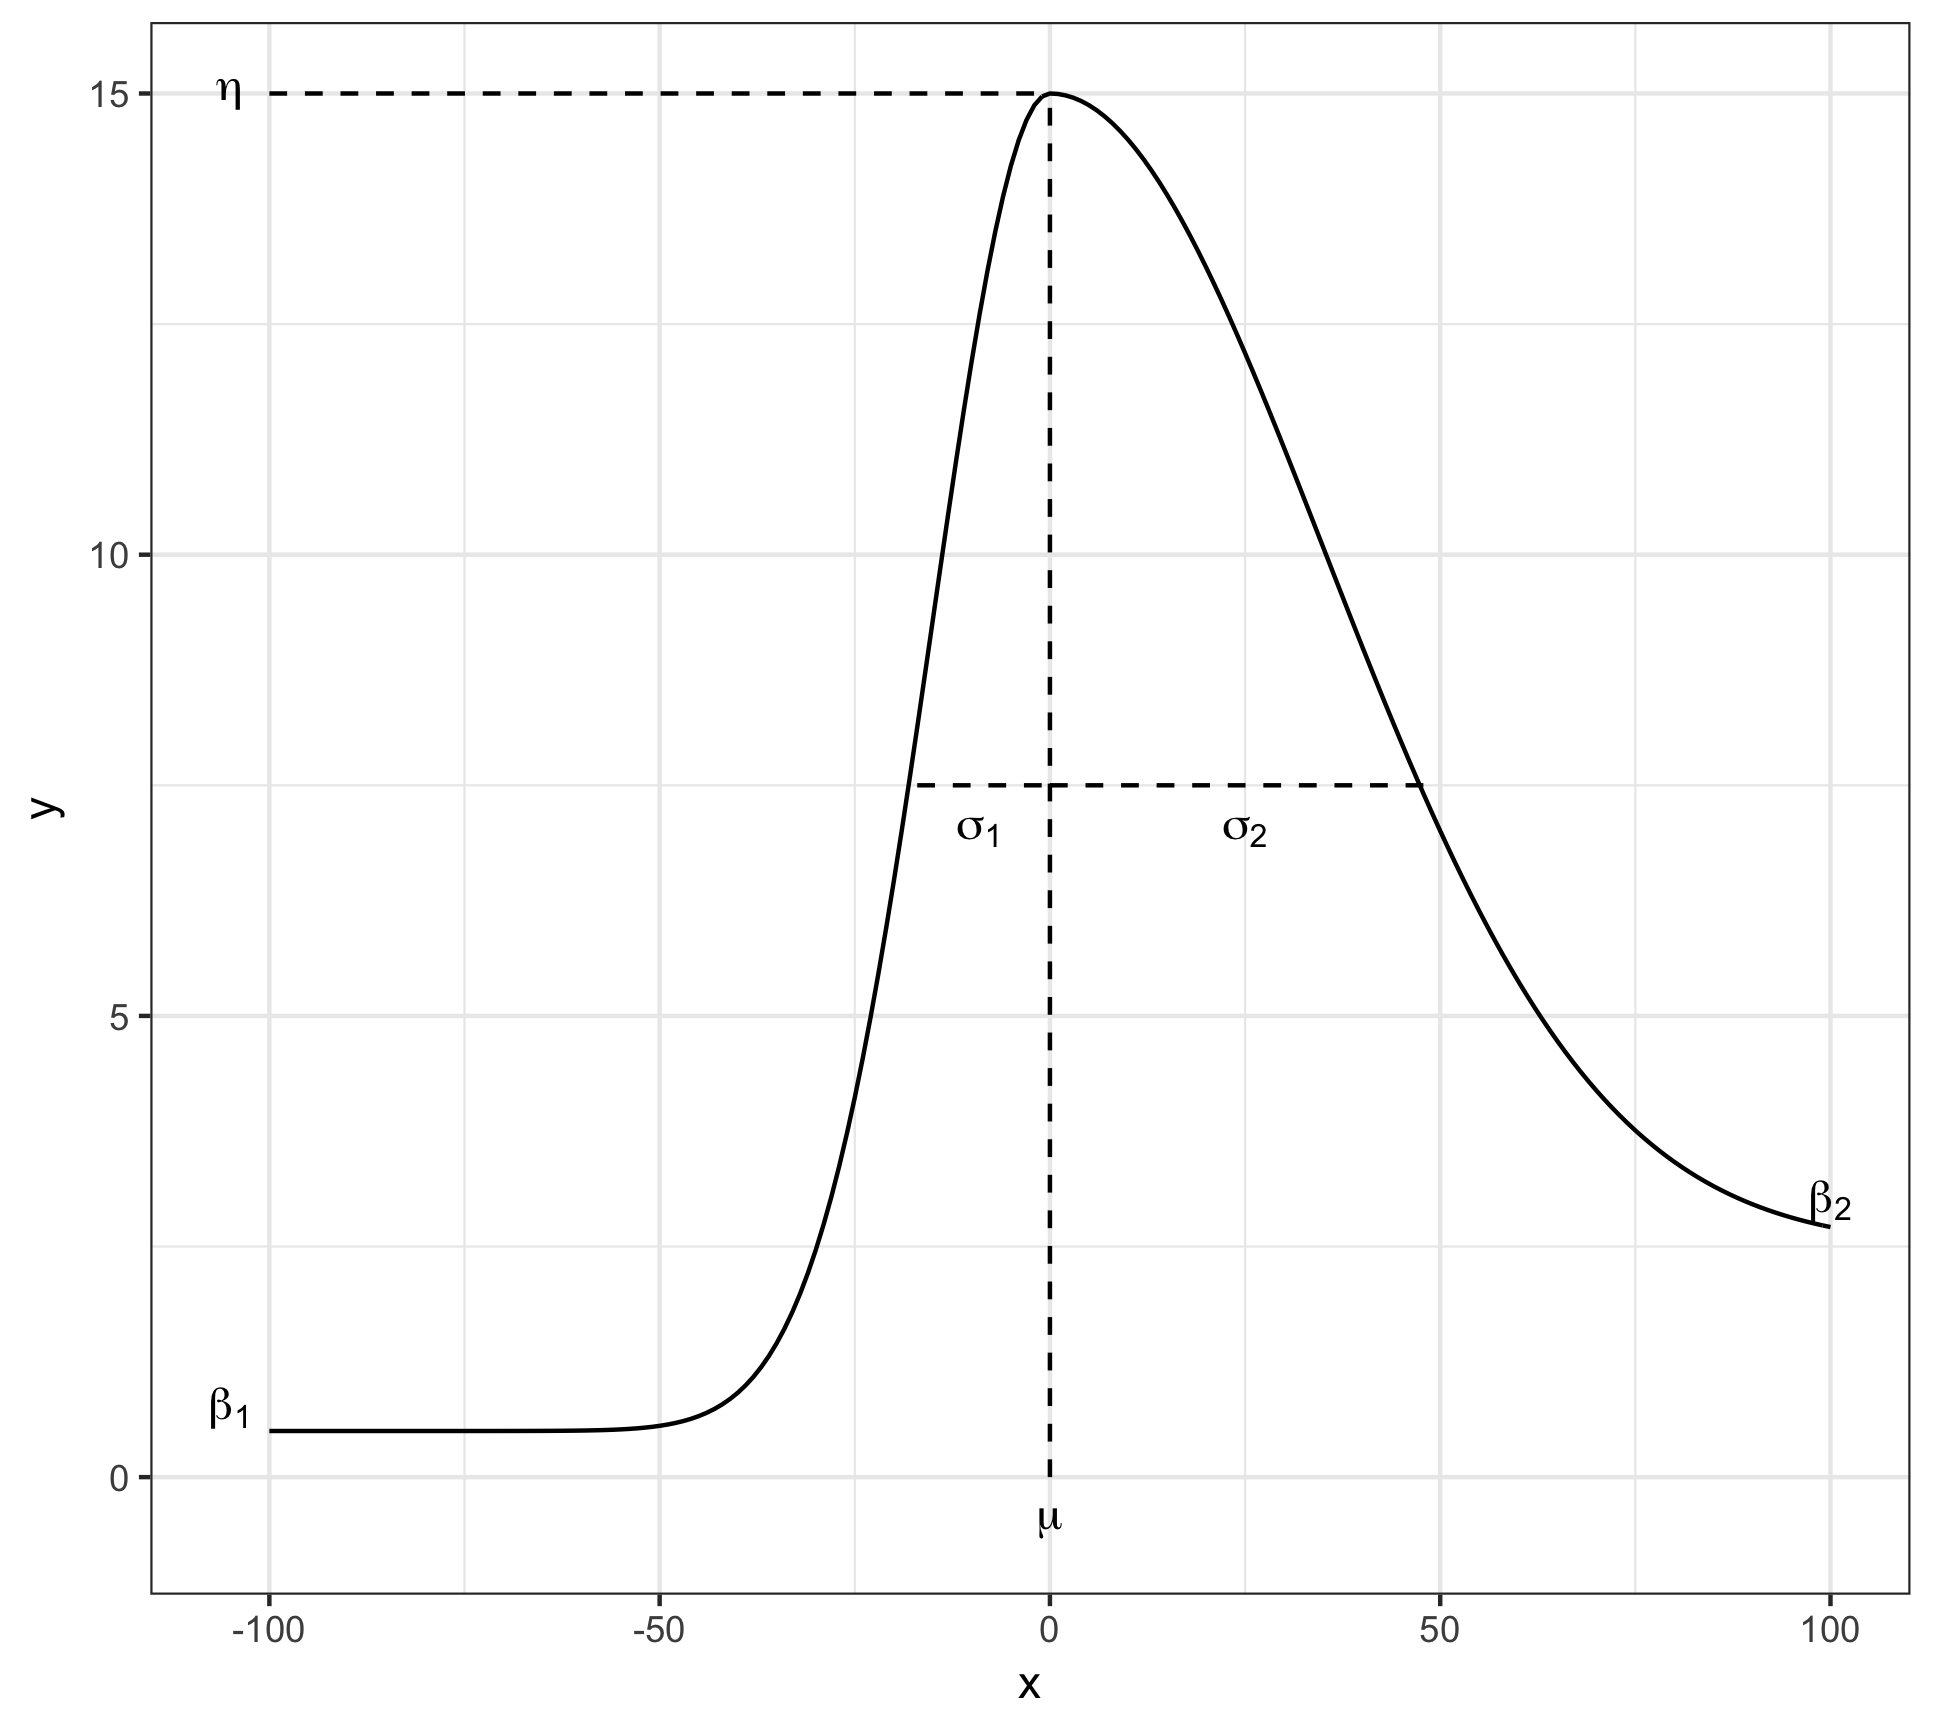
\includegraphics[width=0.70\linewidth]{Figures/ASGFunctFormPlot.png}
  % \caption{%Plot of the Asymmetrical Gaussian curve and its parameters placed according to their corresponding aspects.
  % }
  % \label{fig:ASGff}
\end{figure}

\end{frame}


%%%%%%%%%%%%%%%%%%%%%%%%%%%%%%%%%%%%
%%%%%%%%%%%% Benefits %%%%%%%%%%%%%%
%%%%%%%%%%%%%%%%%%%%%%%%%%%%%%%%%%%%

\section{Beneficial Ideas}
\begin{frame}
\frametitle{Beneficial Practices}

\begin{itemize}
\item Empiracal Bayes to speed up computation
\item Hierarchy structures are beneficial
\item Automate as much as possible
\end{itemize}

\end{frame}




\end{document}
